\chapter{Differential Analysis}

\section{Mass Conservation}
{\footnotesize\textit{Munson 6.2}}
Recall the law for mass conservation that was transferred to a control volume approach in the last chapter:
\begin{equation*}
	\begin{split}
		\frac{dM_{sys}}{Dt}&=0\\
		\text{\footnotesize Reynolds Transport Theorem:} \quad \frac{\partial}{\partial t}\int_{cv} \rho \,dV + \underbrace{\int_{cs} \rho \vec v \cdot \hat n\,dA}_{\stackrel{\text{Gauss}}{=} \int_{cv} \nabla \cdot (\rho \vec v )\,dV} &= 0\hfill\\
		\int_{cv} \left[\frac{\partial}{\partial} \rho + \nabla \cdot (\rho \vec v)\right]\,dV &= 0 \stackrel{(*)}\Longleftrightarrow \frac{\partial}{\partial} \rho + \nabla \cdot (\rho \vec v)=0
	\end{split}
\end{equation*}
Where at $(*)$ we figure that an integral over an arbitrary volume can only be zero if the integrand itself is zero.
The resulting equation is what we call the \textbf{continuity equation}:
\begin{equation*}
	\boxed{\frac{\partial \rho}{\partial t} + \nabla \cdot \left(\rho \vec v \right) = 0}\qquad \text{Eularian Form}
\end{equation*}
The Lagrangian form is as follows:
\begin{equation*}
	\boxed{\frac{D\rho}{Dt} + \rho \nabla \cdot \vec v = 0} \qquad \text{Lagrangian Form}
\end{equation*}

For an incompressible case, where $\rho = const$, then 
\begin{equation*}
	\boxed{\nabla \cdot \vec v = 0}  \qquad \text{Incompressible}
\end{equation*}




\section{Navier-Stokes Equations (Momentum Conservation / Newtons \nth2 law)}
{\footnotesize\textit{Munson 6.3}}  Recall newtons \nth2 law for a Lagrangian system, which we rewrote to an eularian fashion:
\begin{equation*}
	\frac{D}{Dt} (M\vec v)_{sys} = \sum \vec F_{ext}\implies \frac{\partial}{\partial t} \int_{cv}\rho\vec v \,dV + \int_{cs}\rho \vec v (\vec v \cdot \hat n) = \sum \vec F_{ext}
\end{equation*}
As before, we would like to rewrite everything under one volume integral. 

The second term can be rewritten using Gauss:
\begin{equation*}
	\int_{cs} \rho \vec v(\vec v \cdot \hat n) \,dA \stackrel{\text{Gauss}}{=} \int_{cv} \nabla\cdot (\vec v \rho \vec v)\,dV
\end{equation*}
Since $\rho$ is constant, we can denote the $i$th component of the integrand as 
\begin{equation*}
	\nabla\cdot (\vec v \rho \vec v)\stackrel{\nabla \cdot \vec v = 0}= \rho v_j \partial_j v_i = \rho \vec v \cdot \nabla \vec v
\end{equation*}

For a control volume, we want to consider the following forces (right hand term):
\begin{itemize}
	\setlength{\itemsep}{-5pt}
	\item \textbf{body forces}
	\begin{equation*}
		\int_{cv} \rho \vec g \,dV
	\end{equation*}
	\item \textbf{surface forces} (including non-viscous forces)
	
	The non-viscous force is pressure acting on the differential element. non-viscous forces are represented in the rank two stress tensor $\overline{\overline{\tau}}$:
	\begin{equation*}
		\overline{\overline{\tau}} = \begin{pmatrix}
			\tau_{xx}&\tau_{xy}&\tau_{xz}\\
			\tau_{yx}&\tau_{yy}&\tau_{yz}\\
			\tau_{zx}&\tau_{zy}&\tau_{zz}\\
		\end{pmatrix}
	\end{equation*}
	The stress tensor has the following properties:
	\begin{itemize}
		\item $\hat n \cdot \overline{\overline{\tau}}$ or $(\hat n \cdot \overline{\overline{\tau}})_j = n_i\tau_{ij}$ is the stress on the surface with normal $\hat n$.
		\item $\tau_{ij} = \tau_{ji}\implies \hat n \cdot \overline{\overline{\tau}}  = \overline{\overline{\tau}} \hat n$ (symmetric)
	\end{itemize}
	We define the cauchy stress tensor $\overline{\overline \sigma}\cdot \hat n$ with $\overline{\overline \sigma} = -p\overline{\overline{I_d}} + \overline{\overline{\tau}}$ All surface forces combined can therefore be expressed as
	\begin{equation*}
		\int_{cs} \overline{\overline \sigma }\cdot \hat n  \,dA = \int_{cv} \nabla \cdot \overline{\overline {\sigma}}\,dV
	\end{equation*}
\end{itemize}

The complete volume integral with all terms is
\begin{equation*}
	\int_{cv}\rho\frac{\partial \vec v}{\partial t} + \rho \vec v \cdot \nabla \vec v - \rho \vec g - \nabla \cdot (-p\overline{\overline{I_d}}+ \overline{\overline{\tau}}) \,dV = 0
\end{equation*}
Which is valid for all control volumes, and therefore the integrand must also be zero. This is the \textbf{Cauchy's Equation}:
\begin{equation}
\boxed{\rho \left(\frac{\partial \vec v}{\partial t} + \vec v \cdot \nabla \vec v \right) =-\nabla p + \rho \vec g + \nabla \cdot \overline{\overline{\tau}}}
\end{equation}



Recall the result for a Newtonian fluid:
\begin{equation*}
	\tau = \mu \frac{dv_x}{dy} = \tau_{yx}=\tau_{xy}
\end{equation*}
We now know that this $\tau$ is a component of the stress-strain tensor $\overline{\overline{\tau}}$. We were looking at the surface $y$ in the velocity in $x$. We can therefore express the stress-strain rate relationship (which is linear) for a more complicated geometry, as
\begin{equation*}
	\tau_{ij} = \mu \left(\frac{\partial v_i}{\partial x_j} + \frac{\partial v_j}{\partial x_i}\right)
\end{equation*}

Through this new relation, we can substitute into Cauchy's Equation:
\begin{equation*}
	(\nabla \cdot \overline{\overline{\tau}})_j = \partial_i\tau_{ij} = \mu \left(\cancel{\partial_i\partial_j v_i} + \partial_i \partial_i v_j\right) = \mu \nabla^2v_j
\end{equation*}
We could cancel the first term due to mass conservation for incompressible fluids ($\nabla \cdot \vec v = 0$).
this yields

\resizebox{\textwidth}{!}{\shadowbox{$\displaystyle
		{\boxed{\rho \left(\frac{\partial \vec v}{\partial t} + \vec v \cdot \nabla \vec v \right) =-\nabla p + \rho \vec g + \mu \nabla^2\vec v}} \qquad \substack{\text{Navier-Stokes Equation}\\\text{(Incompressible flow)}}
		$}}
	
For an incompressible Newtonian fluid with $\rho = const, \mu = const$, 
we can summarise:
\begin{equation*}
	\begin{cases}
		\rho \left(\frac{\partial \vec v}{\partial t} + \vec v \cdot \nabla \vec v \right) =-\nabla p + \rho \vec g + \mu \nabla^2\vec v\\
		\nabla \cdot \vec v = 0
	\end{cases}
\end{equation*}
Together with boundary and initial conditions, this describes all fluid mechanics problems of Newtonian fluids.
We cannot solve it however.

In order to make progress, we can solve it for a set of special cases.
  
\section{Inviscid Flow}
Looking at the Navier-Stokes Equation, we want to find out in which cases it is okay to neglect the inertial term and the viscous term:
\begin{equation*}
	\rho \frac{\partial \vec v}{\partial t} + \underbrace{\cancel{\rho \vec v \cdot \nabla \vec v}}_{\substack{\text{inertial /}\\\text{advection term}}}  = -\nabla p + \rho g + \underbrace{\cancel{\mu \nabla^2 \vec v}}_{\substack{\text{viscous}\\\text{term}}}
\end{equation*}
We want to understand the "scaling" in order to estimate the terms:
\begin{itemize}
	\setlength{\itemsep}{-5pt}
	\item \textbf{viscous term:} $|\mu\nabla^2 \vec v| \approx \mu \cdot \frac{V}{L^2}$
	\item \textbf{inertial term:} $|\rho \vec v \cdot \nabla \vec v|\approx \rho \cdot \frac{V^2}{L}$
\end{itemize}
where $V$ is the characteristic velocity and $L$ is the length.
We define the Reynolds number:
\begin{equation*}
	Re := \frac{\text{"inertial term"}}{\text{viscosity}} = \frac{\rho V^2/L}{\mu V/L^2} = \frac{VL}{\mu/\rho} = \frac{VL}{\nu}
\end{equation*}
where $\nu$ was the kinematic viscosity.
We can conclude that:
\begin{itemize}
	\setlength{\itemsep}{-5pt}
	\item With a \textbf{large Reynolds number} ($Re >> 1$), we can justify to neglect the \textbf{viscous term}\footnote{The term we dropped, we changed the order of the equation from 2 to one: we therefore cannot apply all boundary conditions.}:
	\begin{equation*}
		\boxed{\rho \frac{\partial \vec v}{\partial t} + \rho \vec v \cdot \nabla \vec v =-\nabla p + \rho \vec g }\qquad \substack{\text{Euler Equation}\\\text{"inviscid flow"}}
	\end{equation*}
	\item With a \textbf{small Reynolds number} ($Re << 1$), we can justify to neglect the \textbf{inertial term}
	\begin{equation*}
		\boxed{\rho \frac{\partial \vec v}{\partial t} =-\nabla p + \rho \vec g + \mu \nabla^2\vec v}\qquad \substack{\text{Stoke's Equation}\\\text{"creeping flow"}}
	\end{equation*}
\end{itemize}

\section{Vorticity and Circulation}
\paragraph{Deformation of a Fluid Element:} Let's consider a fluid element as a box with a certain size $\delta x, \delta y, \delta z$. It is advected in the fluid flow. If the velocity would be uniform, then the fluid element would just be transported without deforming. If not (i.e. the corners of the box don't have the same velocity), it will deform. \textit{The deformation is controlled by the velocity gradients with space}.

\begin{itemize}
	\setlength{\itemsep}{-5pt}
	\item \textbf{linear deformation}: (diagonal components of the gradient velocity tensor)
	\begin{figure}[H]
		\centering
		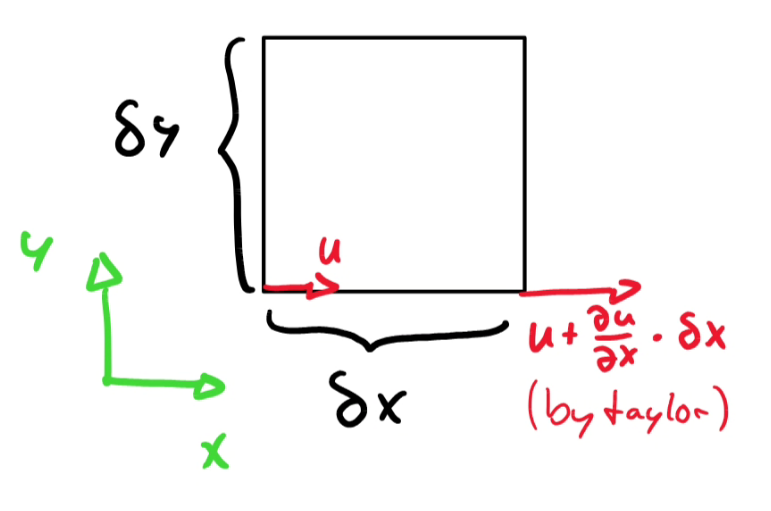
\includegraphics[width=0.4\linewidth]{Sketches/LinearDeformation}
		\caption{}
		\label{fig:lineardeformation}
	\end{figure}
	\begin{equation*}
		\frac{d(\delta x)}{d t} = \frac{\partial u}{\partial x} \implies \frac{1}{\delta x} \frac{d (\delta x)}{d t} = \frac{\partial u}{\partial x}
	\end{equation*}
	Likewise, $\partial_y v, \partial_z w$ are the linear deformations in $y$ and $z$, respectively. The volume change $\delta V = \delta x\cdot \delta y \cdot \delta z $ can be expressed as:
	\begin{equation*}
	\begin{split}
		   \frac{1}{\delta V}\frac{d(\delta V)}{dt}  
		&= \frac{1}{\delta x}\frac{d(\delta x)}{dt} + \frac{1}{\delta y}\frac{d(\delta y)}{dt}+\frac{1}{\delta z}\frac{d(\delta z)}{dt} \\
		&= \frac{\partial u}{\partial x} + \frac{\partial v}{\partial y } + \frac{\partial w}{\partial z}\\
		&= \nabla \cdot \vec v = 0\text{, if $\rho=const$}
	\end{split}
	\end{equation*}
	\item \textbf{angular deformations} (off-diagonal components of the gradient velocity tensor)
	\begin{figure}[H]
		\centering
		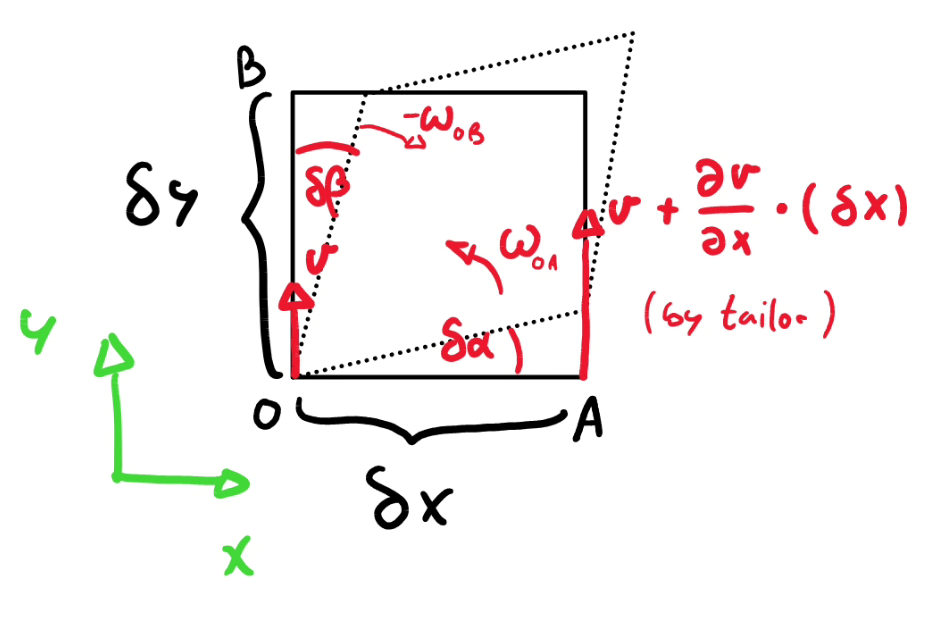
\includegraphics[width=0.4\linewidth]{Sketches/angular_deformations}
		\caption{}
		\label{fig:angulardeformations}
	\end{figure}
	\begin{equation*}
		\begin{split}
			\omega_{OA} &= \lim_{\Delta t \to 0}  \frac{\delta \alpha}{\Delta t} \stackrel{(*)}= \lim_{\Delta t \to 0} \frac{1}{\Delta t} \left(\frac{\frac{\partial v}{\partial x}\delta x \Delta t}{\delta x}\right) = \frac{\partial v}{\partial x}\\
			\omega_{OB} &= -\frac{\partial u}{\partial y}
		\end{split}
	\end{equation*}
	At $(*)$ we used a small angle approximation $\tan\delta \alpha \approx \delta \alpha$. The average rotation is the rotation of the bisecting line $\overline {OC}$. We can write it's angular velocity as
	\begin{equation*}
		\omega_z = \frac 12 \left(\omega_{OA}+\omega_{OB}\right) = \frac 12 \left(\frac{\partial v}{\partial x} - \frac{\partial u}{\partial y}\right)
	\end{equation*}
	Applying the same around $x$ and $y$ axis yields
	\begin{equation*}
		\vec \omega = \frac 12 \nabla \times \vec v = \frac 12 \zeta
	\end{equation*}
	in terms of the is the \textbf{vorticity} $\zeta$:\footnote{Heads up: Vorticity is not necessarily a circular transportation, but rather if (and how much) the fluid elements rotate about \textbf{their own axis}.}
	\begin{equation*}
		\boxed{\zeta = \nabla \times \vec v}
	\end{equation*}
	\textbf{Circularity} is a measure of velocity on some curve $c$ around an area $A$ on the surface of a volume.
	\begin{equation*}
		\Gamma = \oint_{c} \vec v \cdot \vec{ds} = \oint_{A} (\nabla \times \vec v )\cdot \vec{dA}
	\end{equation*}
	Where we see the vorticity again.
	It can be shown that inviscid flow means no change in rotation ($d\Gamma/dt=0$) and we say that "$\Gamma$ is conserved".
	
	It is therefore reasonable to consider inviscid flows ($\mu \to 0$) and irrotational flows ($\nabla \times \vec v = \vec 0$).
\end{itemize}


\section{Potential flow / Irrotational flow}
We assume that we are looking at \textit{incompressible, inviscid, and irrotational} flow.
We know that
\begin{equation*}
	\nabla \times \vec v = \vec 0\implies \exists \phi : \vec v = \nabla \phi
\end{equation*}
with the velocity potential $\phi$.

The continuity, and momentum equations turn into:
\begin{equation*}
	\begin{split}
		\text{Continuity Equation}\qquad\qquad\qquad\qquad\quad \nabla \cdot \vec v &= 0 \qquad (\rho = const) \\
		&\implies \boxed{\nabla^2 \phi = 0}\\\\
		\text{Momentum balance}\qquad\,\,\qquad \rho \left(\frac{\partial \vec v}{\partial t}+ \vec v \cdot \nabla \vec v \right) &= \rho \vec g - \nabla p \qquad \\
		\implies  \rho \frac{\partial \phi}{\partial t} + \frac{\rho}{2}v^2 + p + \rho g z &= const \qquad \Big | \text{steady:} \partial_t \phi = 0\\		
		\frac{\rho}{2}v^2 + p + \rho g z &= const
	\end{split}
\end{equation*}
Note that the result from the momentum balance is the same as the Bernoulli equation, but not restricted to any field lines.

To solve such a problem we follow the following steps:
\begin{enumerate}
	\setlength{\itemsep}{-5pt}
	\item \textbf{Solve Laplace} $\nabla^2\phi = 0$ with appropriate boundary conditions
	\item \textbf{Compute Velocity} $\vec v = \nabla \phi\implies \phi, \vec v$ known
	\item \textbf{Solve for the Pressure} Solve the momentum balance $\frac{\rho}{2}v^2 + p + \rho g z = const$ for pressure.
	\item \textbf{Integrate Pressure over Surface} to get the force on the object
\end{enumerate}


\section{2D Flows -- The Stream Function}
We start from the conservation of mass in an incompressible situation:
\begin{equation*}
	\begin{split}
		\nabla \cdot \vec v &= 0, \vec v = u\hat i + v\hat j + \cancel{w\hat k}\\
		\nabla \cdot \vec v &= 0 \Leftrightarrow \frac{\partial u}{\partial x} = - \frac{\partial v }{\partial y}\\
		\exists \Psi(x,y) :  \frac{\partial \Psi}{\partial y} &= u, -\frac{\partial \Psi}{\partial x} = v\implies \nabla \vec v = \frac{\partial}{\partial x}\frac{\partial \Psi}{\partial y} - \frac{\partial}{\partial y} \frac{\partial \Psi}{\partial x} = 0
	\end{split}
\end{equation*}
If we have a 2D-velocity field which is derived from a so-called \textbf{Stream Function} $\Psi$, it automatically satisfies mass conservation.

To observe places, where the $\Psi$ is constant, the exact differential of $\Psi$ can be expressed as:
\begin{equation*}
	d\Psi = \frac{\partial \Psi}{\partial x}\cdot dx + \frac{\partial \Psi}{\partial y}\cdot dy = 0\Leftrightarrow \frac{dy}{dx} = \frac{v}{u}\quad \text{eq. of a streamline}
\end{equation*}
Therefore, a stream function is constant along a stream line.

\section{2D Potential Flow}
If we assume the following things
\begin{itemize}
	\setlength{\itemsep}{-5pt}
	\item incompressible
	\item inviscid
	\item irrotational $\implies \vec v = \nabla \phi$
	\item 2d $\implies $ there is a stream function $\Psi$
\end{itemize}
We can therefore combine
\begin{equation*}
	\begin{split}
		\phi:\qquad 0 &= \nabla \cdot \vec v = \nabla^2 \phi \\
		\implies 0&=\frac{\partial^2 \phi}{\partial x^2}+ \frac{\partial ^2 \phi}{\partial y^2} \\
		\Psi: \qquad \vec 0 &= \nabla \times \vec v\\\implies 0 &= \frac{\partial ^2 \psi}{\partial x^2}+ \frac{\partial ^2 \psi}{\partial y^2}
	\end{split}
\end{equation*}
Both the stream function and the velocity potential satisfy the Laplace equation\footnote{They don't need to be the same yet, as the boundary conditions are not clear.}

To compare them, we compare their differential:
\begin{equation*}
	d\phi  = u dx + v dy = 0\implies \frac{d y}{dx} = -\frac{u}v
\end{equation*}
the slope is the negative inverse of the stream function, meaning they are orthogonal to the stream lines. From this follows that:

\shadowbox{Equipotential lines ($\phi = const$) are perpendicular to stream lines ($\psi = const$).}

\begin{figure}[H]
	\centering
	\begin{subfigure}{0.48\linewidth}
		\centering
		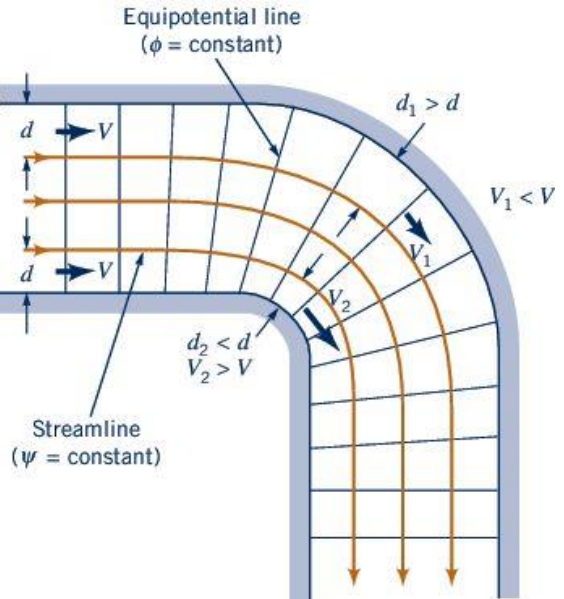
\includegraphics[height=5cm]{Sketches/equipotential_lines_1}
		\caption{streamline and equipotential line illustrated around a curve}
		\label{fig:equipotentiallines1}
	\end{subfigure}%
	\hfill
	\begin{subfigure}{0.48\linewidth}
		\centering
		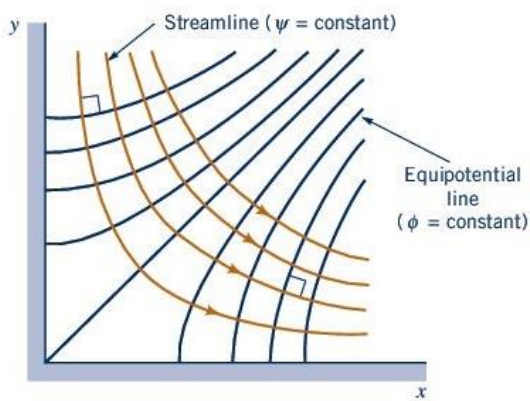
\includegraphics[height=5cm]{Sketches/equipotential_lines_2}
		\caption{streamline and equipotential line illustrated in a corner}
		\label{fig:equipotentiallines2}
	\end{subfigure}
\end{figure}

\paragraph{Example}
Given $\phi = \frac a2 (x^2-y^2)$, we calculate $\partial^2_{xx}\phi + \partial^2_{yy}\phi = a-a = 0$ to verify that it satisfies the condition for a velocity potential. We can den try to determine the stream function $\psi$, by their relationship via $u$ and $v$:
\begin{equation*}
	\left.\begin{split}
		u &= \frac{\partial \phi}{\partial x} = ax = \frac{\partial \psi}{\partial y}\\
		v &= \frac{\partial \phi}{\partial y} = -ay = -\frac{\partial \psi}{\partial x}
	\end{split}\right\} \Psi = axy + \cancel c
\end{equation*}
The constant has no physical meaning, and can be chosen arbitrarily (zero is the simplest one choice.)




\subsection{Basic plane potential flows}
If we can construct a potential-flow solution, such that the stream line captures a desired surface of a 2D body, then boundary conditions are satisfied on the surface. These flow solutions can be superimposed to get more complex solutions.

We will discuss four flows
\subsubsection{Uniform Flow}
\begin{equation*}
	\begin{split}
		\phi &= U_0\cdot x\\
		\psi &= U_0\cdot y
	\end{split}
\end{equation*}
\begin{figure}[H]
	\centering
	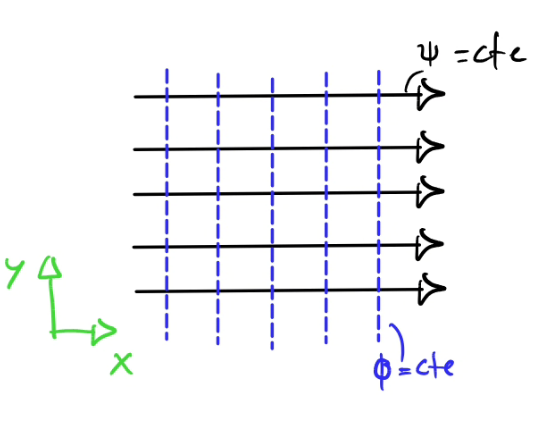
\includegraphics[width=0.4\linewidth]{Sketches/uniform_flow}
	\caption{}
	\label{fig:uniformflow}
\end{figure}

\subsubsection{Line-Source and -Sink}
At a point in space (here the origin), a volume rate $m$ is emerging. 
\begin{equation*}
	\left.\begin{split}
		v_r&= \frac{m}{2\pi r} =  \frac{\partial \phi}{\partial r} = \frac 1r \frac{\partial \Psi}{\partial \theta}\\
		v_\theta &= 0 = \frac 1r \frac{\partial \phi}{\partial \theta} = -\frac{\partial \Psi}{\partial r}
	\end{split}\right\}\implies \begin{cases}
	\phi =\frac{m}{2\pi}\ln r \\
	\psi = \frac{m}{2\pi}\theta
	\end{cases}\hfill
\end{equation*}
\begin{figure}[H]
	\centering
	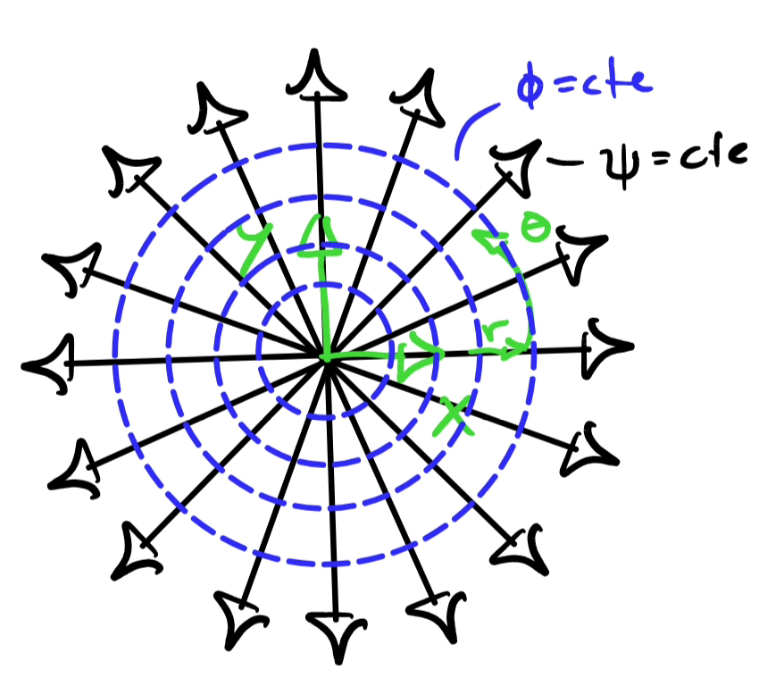
\includegraphics[width=0.4\linewidth]{Sketches/source_sink_flow}
	\caption{}
	\label{fig:sourcesinkflow}
\end{figure}


\subsubsection{Line Vortex}
\begin{equation*}
	\left.\begin{split}
		v_\theta&= \frac{m}{2\pi r} =  \frac 1r \frac{\partial \phi}{\partial \theta} = -\frac{\partial \Psi}{\partial r}\\
		v_r &= 0 = \frac{\partial \phi}{\partial r} = \frac 1r \frac{\partial \Psi}{\partial \theta}
	\end{split}\right\}\implies \begin{cases}
		\phi =k\theta \\
		\psi = -k\ln r
	\end{cases}\hfill
\end{equation*}
\begin{figure}[H]
	\centering
	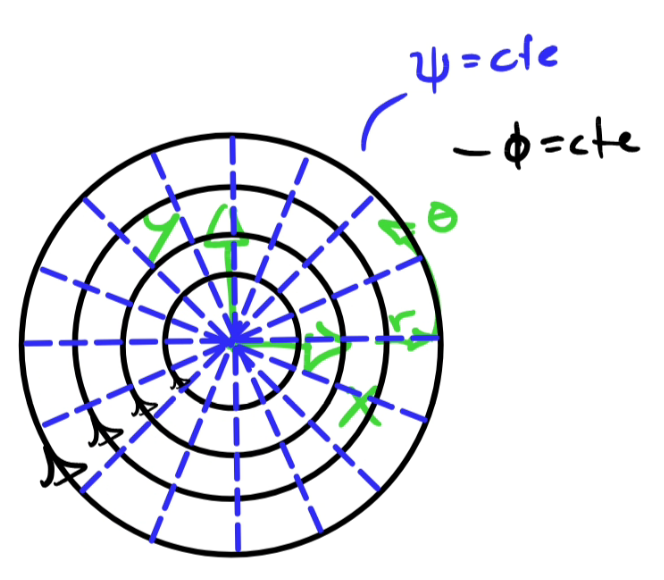
\includegraphics[width=0.4\linewidth]{Sketches/line_vortex_flow}
	\caption{}
	\label{fig:linevortexflow}
\end{figure}

\subsubsection{Doublet}
This is actually already a superposition. Combining a source and a sink at equal distance from the origin of opposite but equal strength. To neglect angular problems, we look at the case where the distance $a$ goes to zero, and the volume rate $m$ to infinity, such that $m\cdot a = const$.
\begin{equation*}
	\begin{split}
		\phi = -\frac{m}{2\pi}(\theta_1-\theta_2) &\stackrel{a\to 0}{\longrightarrow}\frac{k\cos\theta}r\\
	\psi &\stackrel{a\to 0}{\longrightarrow} -\frac{k\sin\theta}{r}
	\end{split}\qquad k = \frac{ma}{\pi}
\end{equation*}

\begin{figure}[H]
	\centering
	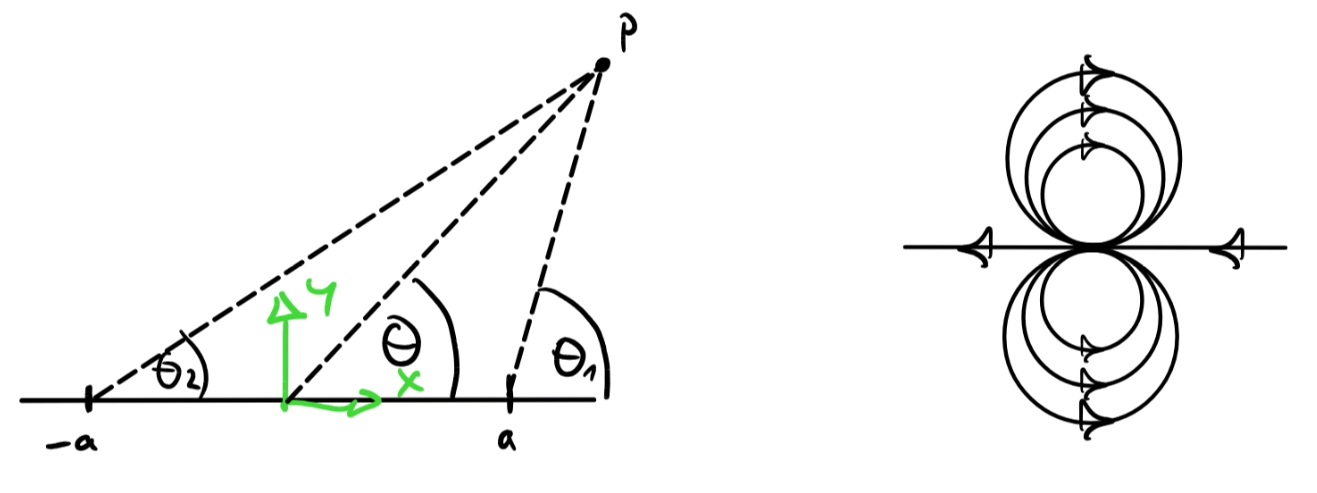
\includegraphics[width=0.4\linewidth]{Sketches/doublet_flow}
	\caption{}
	\label{fig:doubletflow}
\end{figure}
\begin{tabular}{|m{2cm}|l|l|m{4cm}|}
	\hline
	\textbf{Description of Flow Field} & \textbf{Velocity Potential} & \textbf{Stream Function} & \textbf{Velocity Components} \\
	\hline
	Uniform flow at angle $\alpha$ with the $x$ axis &
	$\phi = U(x \cos \alpha + y \sin \alpha)$ &
	$\psi = U(y \cos \alpha - x \sin \alpha)$ &
	$u = U \cos \alpha$ \newline $v = U \sin \alpha$ \\
	\hline
	Source or sink \newline $m > 0$ source \newline $m < 0$ sink &
	$\phi = \dfrac{m}{2\pi} \ln r$ &
	$\psi = \dfrac{m}{2\pi} \theta$ &
	$v_r = \dfrac{m}{2\pi r}$ \newline $v_\theta = 0$ \\
	\hline
	Free vortex \newline $\Gamma > 0$ counterclockwise \newline $\Gamma < 0$ clockwise &
	$\phi = \dfrac{\Gamma}{2\pi} \theta$ &
	$\psi = -\dfrac{\Gamma}{2\pi} \ln r$ &
	$v_r = 0$ \newline $v_\theta = \dfrac{\Gamma}{2\pi r}$ \\
	\hline
	Doublet &
	$\phi = \dfrac{K \cos \theta}{r}$ &
	$\psi = -\dfrac{K \sin \theta}{r}$ &
	$v_r = -\dfrac{K \cos \theta}{r^2}$ \newline $v_\theta = -\dfrac{K \sin \theta}{r^2}$ \\
	\hline
\end{tabular}
\subsection{Superpositions}
\subsubsection{The Half-Body}
This is a superposition of a source and a uniform flow.
Through linearity, the stream function for this combination is:
\begin{equation*}
	\begin{split}
		\psi &= \psi_{UF} + \psi_{S}\\
		&= U_0\cdot y + \frac{m}{2\pi}\theta \\
		&= U_0r\sin\theta + \frac{m}{2\pi}\theta
	\end{split}
\end{equation*}
The velocity potential $\phi$ can be described similarly through
\begin{equation*}
	\begin{split}
		\phi &= \phi_{UF} + \phi_{S}\\
		&=U_0r\sin\theta + \frac{m}{2\pi}\ln r 
	\end{split}
\end{equation*}

Through these definitions of $\phi$ and $\psi$, we can express the velocities as follows:
\begin{equation*}
	\begin{split}
		v_r &= \frac 1r \frac{\partial \psi}{\partial \theta } = U_0 \cos\theta + \frac{m}{2\pi r}\\
		v_\theta &= - \frac{\partial \psi}{\partial r} = -U_0\sin\theta 
	\end{split}
\end{equation*}

To understand these velocities, we find the stagnation point on the x-axis, at $\theta_{sp}=\pi$, $v_r= 0$:
\begin{equation*}
	0=u_0\cos\theta_{sp} + \frac{m}{2\pi r_{sp}} \implies r_{sp} = \frac{m}{2\pi U_0}
\end{equation*}
\begin{figure}[H]
	\centering
	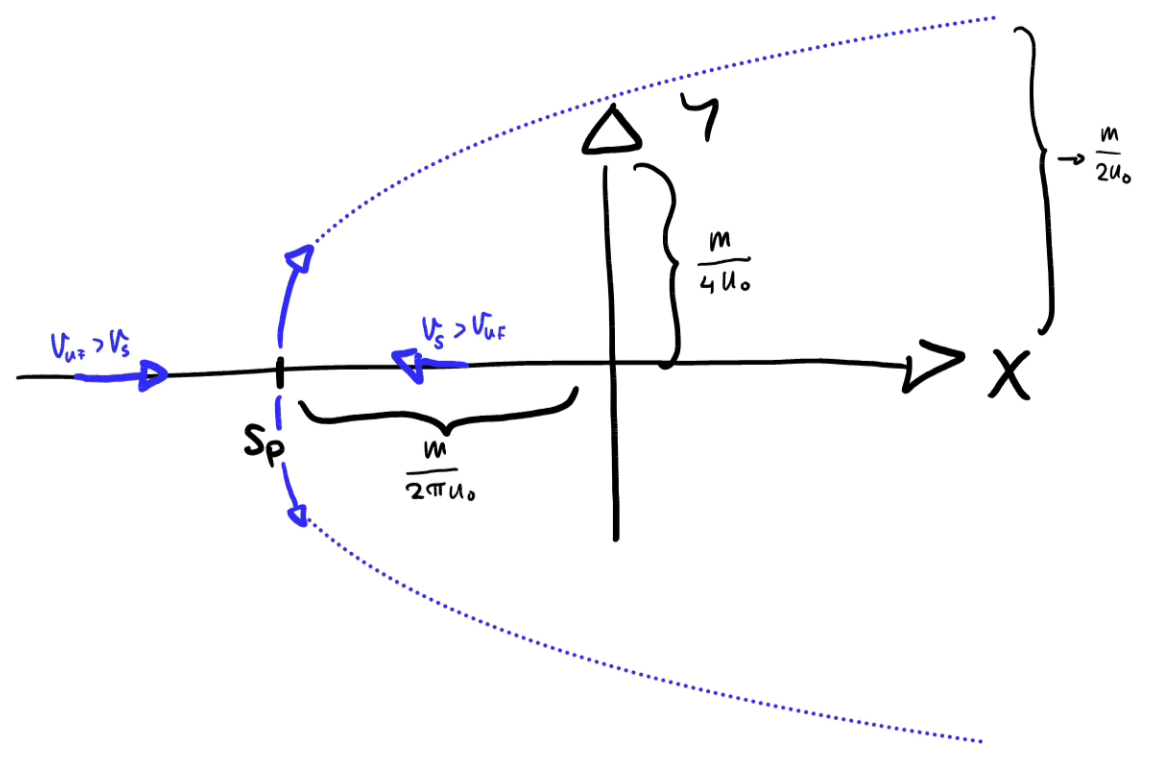
\includegraphics[width=0.4\linewidth]{Sketches/halfbody}
	\caption{}
	\label{fig:halfbody}
\end{figure}
Describing the stagnation stream line, we write
\begin{equation*}
	\psi_{sp} = \frac m2 = U_0 r \sin\theta + \frac{m}{2\pi}\theta \implies r = \frac{m}{2\pi U_0} \frac{\pi - \theta}{\sin\theta},\quad \theta \in[0,2\pi[
\end{equation*}

The intersection point of the stagnation stream line on the $y$ axis is at $\theta=\pi/2$, with radius $r=\frac{m}{4U_0}$.
To inspect the y-height of the stagnation stream line, we get $y=r\sin\theta = \frac{m}{2\pi U_0}(\pi-\theta) = \frac{m}{2 U_0}$.

We interpret the stagnation stream line as the surface of a so-called \textit{half-body}.

Next we would like to calculate the velocity and pressure on the surface
\begin{equation*}
	v^2 + v_r^2 + v_\theta ^2 = U_0^2 \left(1+2\frac{b}{r}\cos(\theta) + \frac{b^2}{r^2}\right), \qquad b = \frac{m}{2\pi U_0}
\end{equation*}

\subsubsection{Rankine Oval}
A source and sink placed at $x=-a$ and $x=a$ respectively, all inside of a uniform flow. This will not be discussed, further reference can be found in \textbf{Munson 6.6.2}.

\subsubsection{Circular Cylinder}
We superimpose uniform flow and a doublet. We can immediately write the stream function and velocity potential
\begin{equation*}
	\begin{split}
		\psi &= \psi_{UF} + \psi_{D} = U_0y - \frac{K\sin\theta}{r} = \left(U_0+\frac{K}{r^2}\right)r\sin\theta\\
		\phi &= \phi_{UF} + \phi_D = \left(U_0+\frac K{r^2}\right)r\cos\theta
	\end{split}
\end{equation*}

We have two stagnation points for $y=0$, $\theta\in\{0,\pi\}$. $\psi=0$ is a stream line through $r=a$ if $u_0-\frac K{r^2}=0$. We need to choose $K=U_0a^2$, such that the stagnation stream line is a circle with radius $a$. The flow around a cylinder of radius $a$ can be described as:
\begin{equation*}
	\begin{split}
		\psi = U_0 \left(1-\frac{a^2}{r^2}\right) r \sin\theta\\
		\phi = U_0 \left(1+\frac{a^2}{r^2}\right)r \cos\theta
	\end{split}
\end{equation*}

The velocity can be written as
\begin{equation*}
	\begin{split}
		 v_r &= \frac{\partial \phi}{\partial r} = \frac{1}{r}\frac{\partial \psi}{\partial \theta }=U_0\left(1-\frac{a^2}{r^2}\right)\cos\theta\\
		 v_\theta &= \frac{1}{r}\frac{\partial \phi}{\partial \theta} = -\frac{\partial \psi}{\partial r} = - U_0\left(1+\frac{a^2}{r^2}\right) r \sin\theta
	\end{split}
\end{equation*}
On the surface of the cylinder ($a=r$), we get $v_r = 0$ and $v_\theta = 2a \sin\theta$. This is okay, as the flow is assumed to be inviscid. 

To calculate the pressure $p_s$ on the surface, we use newton's second law:
\begin{equation*}
	\begin{split}
		\rho \frac{\partial \phi}{\partial t}+ \frac{\rho}{2}|\vec v|^2 + p + \cancel{\rho gz}^{\text{negl.}} &= const\\
		p_0 + \frac 1 2\rho U_0^2 &= p_s + \frac 12 \rho v_{\theta}^2\\
		\implies p_s&=p_0 + \frac 12 \rho U_0^2\left(1-4\sin^2\theta\right)
	\end{split}
\end{equation*}
\paragraph{Drag and Lift Forces}
\begin{equation*}
	\begin{split}
		F_L &= F_y = -\int_0^{2\pi}p_s\sin\theta a\,d\theta = 0\implies\text{no lift}\\
		F_D & =F_x =  \int_0^{2\pi}p_s\cos\theta a \,d\theta = 0 \implies \text{no drag}
	\end{split}
\end{equation*}
The result of no drag is called d'Alembert's Paradox and is only true because we assume inviscid flow. For real-world scenarios, the effects of viscosity result in a non-zero drag force. 

\subsubsection{Rotating Cylinder}
In order to create lift, the up-down symmetry needs to be broken. Adding a vortex helps doing this.
\begin{equation*}
	\begin{split}
		\psi &= U_0\left(1-\frac{a^2}{r^2}\right)r\sin\theta - \frac \Gamma {2\pi}\ln r\\
		\phi &= U_0\left(1+\frac{a^2}{r^2}\right)r\sin\theta - \frac \Gamma {2\pi} r\\
	\end{split}
\end{equation*}
On the surface ($r=a$), the velocity becomes:
\begin{equation*}
	\begin{split}
		v_{r,s} = \frac{1}{r}\frac{\partial \psi}{\partial \theta}\Big|_{r=a} = 0\\
		v_{\theta,s} &= -\frac{\partial \psi}{\partial r} \Big|_{r=a} = -2U_0 \sin\theta + \frac{\Gamma}{2\pi a}
	\end{split}
\end{equation*}
At the stagnation point on the cylinder surface, 
\begin{equation*}
	\sin\theta_{sp} = \frac{\Gamma}{2\pi U_0 a}
\end{equation*}
This describes the following points:
\begin{figure}[H]
	\centering
	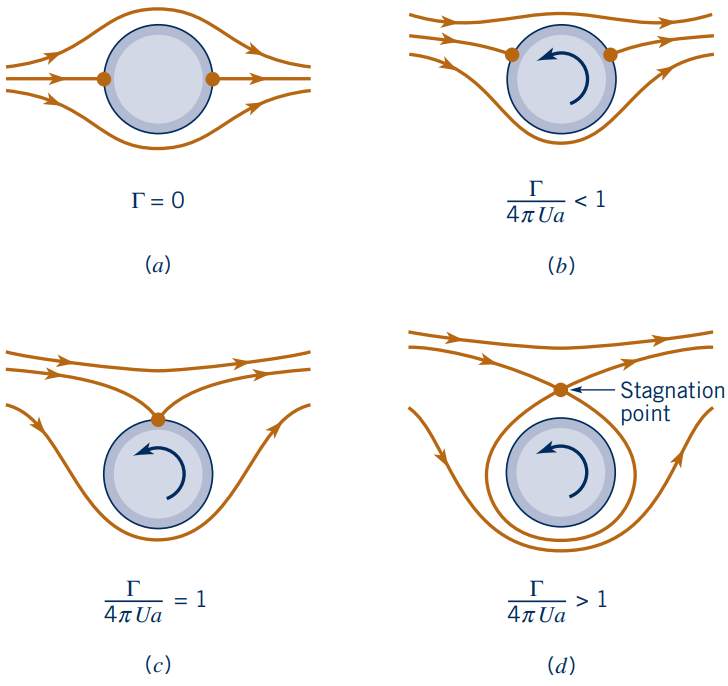
\includegraphics[width=0.4\linewidth]{Sketches/rotating_cylinder_stagnation_points}
	\caption{Munson et.al.}
	\label{fig:rotatingcylinderstagnationpoints}
\end{figure}
The pressure on the surface is
\begin{equation*}
	p_s = p_1 + \frac 12 \rho U_0^2 \left(1-4\sin^2\theta + \frac{2\Gamma\sin\theta}{2\pi a U_0}-\frac{\Gamma^2}{4\pi^2 a^2 U_0^2}\right)
\end{equation*}
This still has symmetries around $\pi/2, 3\pi/2$, and therefore doesn't generate drag. However, the symmetry from $y$ to $-y$ is broken.
This leads to the following lift force:
\begin{equation*}
	F_L = -\int_0^{2\pi} p_s \sin\theta a\,d\theta= -\frac{1}{2}\rho U_0^2\int_0^{2\pi} \frac{2\Gamma \sin\theta}{2\pi a U_0} - \frac{\Gamma^2}{4\pi^2 a^2 U_0^2}a\sin\theta \,d\theta = -\rho U_0 \Gamma
\end{equation*}
Which is the \textbf{Magnus Effect}:
\begin{equation*}
	\boxed{F_L = -\rho U_0 \Gamma}
\end{equation*}
The lift force (perpendicular to the flow direction) per "span" is given by $-\rho U_0 \Gamma$.
When the flow comes from the left, $\Gamma$ must be negative (clockwise) in order for the lift to be positive.
\subsection{Lift and drag on an Airfoil}
\footnotesize{Munson chapter 9}

An airplane flies at high Reynolds numbers, viscosity can be ignored. For inviscid potential flow and infinite wings (that can therefore be observed in 2D), then the general results:
\begin{equation*}
	\begin{aligned}
		F_L &= -\rho U_0 \Gamma &&\textbf{lift per unit span}\\
		F_D &= 0 && \textbf{d'Alembert's paradox}
	\end{aligned}
\end{equation*}

For any closed curve around the airfoil:
\begin{equation*}
	\Gamma = \oint_c \vec v \cdot \vec{ds}
\end{equation*}
are valid for any shape of airfoil.\footnote{By the Kutta-Joukowski theorem} The Kutta-condition chooses the stagnation point to be pinned at the sharp feature on the trailing edge. This limits the infinite solutions resulting from inviscid flow to the solution chosen in nature, where viscosity is still important at high velocities very close to surfaces. Stalling is when the Kutta-condition can no longer be satisfied and no lift is generated.

\section{Viscous Flow}
Recall the equations for incompressible Newtonian fluids:
\begin{equation*}
\begin{split}
		\rho \frac{\partial \vec v}{\partial t}+ \rho \vec v \cdot \nabla \vec v &= -\nabla p + \rho \vec g + \underbrace{\mu \nabla^2 \vec v }_{\text{Viscous term}}\\
		\nabla \cdot \vec v &= 0
\end{split}
\end{equation*}
Viscosity by itself implies the no-slip condition boundary condition at the walls: 
\begin{equation*}
	\vec v = \vec v_{wall}
\end{equation*}

The above equation is very hard to solve, they are non-linear and thus in general impossible to solve. In few specific cases, we can however find solutions to them.
\subsection{Laminar shear flow between parallel plates}
Consider two parallel plates at distance $h$, where one of them moves at velocity $v_0$. The downstream direction is $\hat x$. 

The assumptions of laminar flow are made, which assumes that the solution is of the form $\vec v (\vec r,t)= u(y,t)\hat i$. It only has a downstream component and only depends on $y$, which is the wall-normal coordinate. 

Under these assumptions, the non-linear term vanishes
\begin{equation*}
	\vec v \cdot \nabla \vec v = u(y,t)\frac{\partial}{\partial x}u(y,t)\hat i = \vec 0
\end{equation*}

Furthermore, we assume that there is a constant prescribed pressure gradient along $x$:
\begin{equation*}
	\frac{\partial p}{\partial x} = cte\qquad \frac{\partial p}{\partial z} = 0
\end{equation*}
plugging this into the continuity equation yields
\begin{equation*}
	\nabla \cdot \vec v = \frac{\partial u}{\partial x} + \frac{\partial v}{\partial y} + \frac{\partial w}{\partial z} = 0
\end{equation*}
The moment conservation equation results in
\begin{equation*}
	\begin{split}
		\rho \frac{\partial u}{\partial t}\hat i + \vec 0 &= - \frac{\partial p}{\partial x}\hat i - \frac{\partial p}{\partial y}\hat j - \rho g\hat j + \mu \left(\frac{\partial^2 }{\partial x^2 }+\frac{\partial^2 }{\partial y^2 }+\frac{\partial^2 }{\partial z^2 }\right)u \hat i\\
		\hat i: \qquad \rho \frac{\partial u}{\partial t}&=-\frac{\partial p}{\partial x}+ \mu \frac{\partial^2 }{\partial y^2}u\\
		\hat j:\qquad 0 &= -\frac{\partial p}{\partial y}-\rho g\\
		\hat k: \qquad 0 &= 0\\\\
		\implies p &= -\rho g y + \frac{\partial p}{\partial x}x + C\\
		&= -\rho g y + c
	\end{split}
\end{equation*}
What is left to solve is
\begin{equation*}
	\rho \frac{\partial u}{\partial t} = \mu \frac{\partial ^2}{\partial y^2}u - \frac{\partial p}{\partial x}
\end{equation*}
We can recognise this as a diffusion equation for momentum density with diffusion coefficient $\mu/\rho = \nu$.

\paragraph{Steady State Solutions}
There are three possible combinations:
\begin{itemize}
	\setlength{\itemsep}{-5pt}
	\item \textbf{plane Poiseuille flow} $u_0=0,\partial_xp \ne 0$\\
	\item \textbf{plane Couette flow} $u_0\ne0 ,\partial_xp =0$\\
	\item \textbf{mixed Couette flow} $u_0\ne0,\partial_xp \ne 0$
\end{itemize}

For each of these, we need to solve
\begin{equation*}
	\begin{cases}
		0=\mu \frac{d^2u}{dy^2}- \frac{\partial p}{\partial x}\\
		u(y=-h) = 0\\
		u(y=h) = u_0
	\end{cases}
\end{equation*}
Which results in 
\begin{equation*}
	\begin{split}
		u &= \frac{1}{2\mu}\left(\frac{\partial p}{\partial x}\right) y^2 + C_1 y + C_2\\\implies
		u(y)&=\frac{u_0}{2}\left(\frac{y}{h} + 1\right)+ \frac{1}{2\mu }\left(\frac{\partial p}{\partial x}\right)\left(y^2 -h^2\right)
	\end{split}
\end{equation*}

The volumetric flow rate (per unit depth) is 
\begin{equation*}
	Q= \int_{-h}^h u\,dy = u_0 h- \frac{2}{\mu} \left(\frac{\partial p}{\partial x}\right)\frac{h^3}{3}
\end{equation*}
\paragraph{Time Dependant Solution}
This can be solved exactly like the diffusion equation. 
\subsection{Pipe Flow}
Assume we have a cylindrical pipe or radius $R$. We impose a cylindrical coordinate system to write the assumptions:
\begin{itemize}
	\setlength{\itemsep}{-5pt}
	\item incompressible,  Newtonian
	\item laminar
	\item steady
	\item $\partial_z p = cte$ (incompressible)
\end{itemize}

From laminar and steady, we conclude
\begin{equation*}
	\begin{split}
		\vec v = V_z (r)\hat z\\
		\nabla \cdot \vec v = 0
	\end{split}
\end{equation*}
the Navier-Stokes equations turn into
\begin{equation*}
	0 = -\partial_zp + \mu \left(\frac 1r \frac{\partial }{\partial r}\left(r \frac{\partial V_z}{\partial r}\right)\right)\\
	\implies V_z = \frac{1}{4\mu}\left(\frac{\partial p}{\partial z}\right) r^2+ c_1\ln r + c_2
\end{equation*}
Through the boundary conditions
\begin{equation*}
	\begin{cases}
		V_z|_{r=R} = 0&(1)\\
		|v_z|_{r=0}< \infty &(2)
	\end{cases}
\end{equation*}
we conclude that by $(1)$ $c_1 = 0$ and by $(2)$:
\begin{equation*}
	c_2 = -\frac{1}{4\mu}\left(\frac{\partial p}{\partial z}\right)R^2
\end{equation*}
and therefore
\begin{equation*}
\boxed{	V_z = \frac{1}{4\mu}\left(\frac{\partial p}{\partial z}\right)(r^2-R^2)}
\end{equation*}